\documentclass{beamer}

\usepackage[utf8]{inputenc}
\usepackage[ngerman]{babel}
\usepackage[T1]{fontenc}

\usepackage{amsmath,amssymb,amsfonts,amsthm,mathtools}

\usepackage{paralist}
\usepackage{bm}
\usepackage{bbm}
\usepackage{algorithm}
\usepackage{algpseudocode}
%\usepackage{algorithm}
%\usepackage{algorithmic}
\usepackage{tikz}
\usepackage{colortbl}

\mode<presentation>
{
  \setbeamertemplate{navigation symbols}{}
    \usetheme{Hannover}
   \setbeamercovered{transparent}
   \useoutertheme{infolines}
}

%\usecaptiontemplate{
%\tiny
%\structure{\insertcaptionname~\insertcaptionnumber:}
%\insertcaption
%}

\title[Simulation einer Populationsdynamik] % (optional, nur bei langen Titeln noetig)
{Simulation einer stochastischen Populationsdynamik}
\subtitle{Vortrag zum Begleitseminars der Bachelorarbeit}
\author[B.Prochnau] % (optional, nur bei vielen Autoren)
{Boris Prochnau}
\institute[Universität Bonn]{Institut für Angewandte Mathematik\\Universität Bonn}

\date {\today}
\setbeamercovered{invisible}

\begin{document}
%
% ****************************************************************************************************
%					preliminaries
% ****************************************************************************************************
%

\begin{frame}
  \titlepage
\end{frame}
\begin{frame}
  \frametitle{Übersicht}
  \tableofcontents
\end{frame}
\section{Einleitung}
\begin{frame}{Einleitung - Was wird simuliert?}
	\begin{minipage}{0.49\textwidth}
		\begin{figure}
		\centering	
		\includegraphics[width=1\linewidth]<3->{./Lizenzbilder/Okosystem1}%
		\includegraphics[width=1\linewidth]<1,2>{./Lizenzbilder/Zelle1}%
		\end{figure}
	\end{minipage}	
	\begin{minipage}{0.49\textwidth}
		\visible<1,2>{{\tiny\textregistered Harald Häck  / pixelio.de}}\\	
		\visible<3->{{\tiny\textregistered Kai Niemeyer  / pixelio.de}}		
		\begin{itemize}
			\item Ein Beute-Beute System mit asexueller Fortpflanzung.\pause
			\item Die Populationsgr"o"se nach Zeit.\pause
			\item Mit abgeschlossenem Ökosystem.\pause
			\item Dabei ist die Populationsdynamik von besonderem Interesse.
		\end{itemize}
	\end{minipage}
\end{frame}
\begin{frame}
	\frametitle{Einleitung - Dynamik durch Wechselwirkung}\pause
	\begin{minipage}{0.49\textwidth}
		\begin{figure}
%		\centering
		\includegraphics[width=1\linewidth]<2>{./Lizenzbilder/Tier5}%
		\visible<2>{\caption{\tiny\textregistered Schnobby / wikimedia.org}}
		\includegraphics[width=1\linewidth]<3>{./Lizenzbilder/Lebensraum1}%
		\visible<3>{\caption{\tiny\textregistered Albedo  / pixelio.de}}
		\includegraphics[width=1\linewidth]<4>{./Lizenzbilder/Pilz2}%
		\visible<4>{\caption{\tiny\textregistered Uschi Dreiucker  / pixelio.de}}		
		\end{figure}
	\end{minipage}
	\begin{minipage}{0.49\textwidth}
		\begin{itemize}		
			\item Z.B. durch unabhängige Nahrungsquellen,\pause
			\item Kampf um Lebensraum,\pause
			\item oder dominantes Ressourcenverhalten.
		\end{itemize}
	\end{minipage}
\end{frame}	
	
\section{Modell}
\begin{frame}{Was enth"alt das Modell?}
\visible<1->{Es enth"alt Individuen mit Merkmalen $ x \in X $.\\}
	\begin{itemize}	
		\item<2-> Arteigene und mutative Geburten.
		\item<3-> Natürliche und wettbewerbliche Tode.
%		\item<4-> Jedem Ereignis kommt eine Ereignisrate zu, welche das Merkmal charakterisieren.
%		\item<5> Diese dienen exponentiellen Ereignisuhren als Parameter.
	\end{itemize}
	\visible<4->{Jedem Ereignis kommt eine Ereignisrate zu, welche das Merkmal charakterisieren.}
	\begin{itemize}
		\item<5-> Diese dienen exponentiellen Ereignisuhren als Parameter.
	\end{itemize}
	\begin{center}\pause\pause\pause\pause\pause
		\begin{tabular}{l | c c | c c}\hline
			direkte Raten: & $ b(x) $ & $ \mu $ \cellcolor{yellow} & $ d(x) $ & $ c(x,y) $\\\pause
			Ereignisraten: & \multicolumn{2}{c|}{$ B(x) $} & \multicolumn{2}{c}{D(x)}\\\hline
		\end{tabular}
	\end{center}
\end{frame}

\begin{frame}{Raten}
	Die zusammengesetzten Raten werden wie folgt gebildet:\bigskip\\
	\begin{minipage}{0.49\textwidth}
		\begin{figure}
		\centering		
		\includegraphics[width=1\linewidth]<2>{./Formelbilder/Birthrate1}%
		\includegraphics[width=1\linewidth]<3>{./Formelbilder/Deathrate1}%
		\includegraphics[width=1\linewidth]<4->{./Formelbilder/TotaleRaten}%
		\end{figure}
	\end{minipage}
	\begin{minipage}{0.49\textwidth}
	\begin{center}
		\begin{itemize}
				\item<2-> Gesamte Geburtenrate aus arteigenen und mutativen Raten.
				\item<3-> Gesamte Todesrate aus nat"urlicher und wettbewerblicher Rate pro Individuum.
				\item<4-> Auf diese selbe Weise lassen sich weitere Ereignisraten formulieren.
		\end{itemize}
	\end{center}
	\end{minipage}
\end{frame}

\begin{frame}
	\frametitle{BPDL-Prozess}
	Die Population ist ein Markov Sprungprozess der durch das folgende Punktma"s beschrieben wird:\pause
	\[ \nu_t = \sum_{i=1}^{N_t} \delta_{x_i}, \text{mit} \int_X 1 \text{ } \nu_t(dx) = N_t \]
	\pause
	Mit dem Generator:
	\begin{flalign*}
		& L(\phi(\nu)) = \sum_{x \in X} b(x)(1-\mu)[\phi(\nu + \delta_{x}) - \phi(\nu)] \cdot n(x)&\\
		& + \sum_{y \sim x}b(x) \cdot \frac{\mu}{2} \cdot 
 		[\phi(\nu + \delta_{y}) - \phi(\nu)] \cdot n(x)&\\		 
		& + \sum_{x \in X} \left(d(x) + \sum_{y \in X} c(x,y) \cdot n(y)\right)[\phi(\nu - \delta_{x}) - \phi(\nu)] \cdot n(x) &
	\end{flalign*}
\end{frame}

\section{Eigenschaften des BPDL-Prozesses}
\subsection{LPA-Normalisierung}
\begin{frame}
	\frametitle{Normalisierung}
\begin{minipage}{0.49\textwidth}
		\begin{figure}
		\centering		
		\includegraphics[width=1\linewidth]<6->{./Lizenzbilder/Normalisierung1}%
		\end{figure}
		\includegraphics[width=1\linewidth]<6->{./Lizenzbilder/Normalisierung3}%
	\end{minipage}
	\begin{minipage}{0.49\textwidth}
		Die LPA Normalisierung erweitert die Betrachtung auf die Ebene der Population.
		\pause
		Dazu:
		\begin{itemize}
			\item<2-> $ \nu_t^K := \frac{1}{K} \nu_t $. 
			\item<3-> $ n_0^K $ wird proportional zu K gewählt. 
			\item<4-> $ b(x), d(x) $ bleiben nat"urlich unver"andert. 
			\item<5-> Jedoch $ c^K(x,y) = \frac{c(x,y)}{K} $.
		\end{itemize}
		\visible<6->{{\tiny \textregistered kaibara87 \\ flickr.com/photos/kaibara/3839720754/\\
		\textregistered Boris Prochnau \\ 
		Moosteppich um Bonsai}
		}	
	\begin{center}
	\end{center}
	\end{minipage}
\end{frame}

\begin{frame}{Normalisierung}
	\begin{minipage}{0.49\textwidth}
		\begin{figure}
		\centering
		\includegraphics[width=1\linewidth]<1,2,3->{./Pictures/Normalisierung1}%
		\\\includegraphics[width=1\linewidth]<1,2,3->{./Pictures/Normalisierung2}%	
%		\includegraphics[width=1\linewidth]<1,2,3->{./Pictures/LPANormalisierungK100}%
%		\\\includegraphics[width=1\linewidth]<1,2,3->{./Pictures/LPANormalisierungK10000}%
		\end{figure}
	\end{minipage}
	\begin{minipage}{0.49\textwidth}
		Bsp. einer LPA-Normalisierung mit $ K = 1 \text{ und } K = 1000 $:
		\begin{itemize}
			\item Flacherer Verlauf der zeitlichen Entwicklung.\pause
			\item Einzelne Ereignisse lassen sich nicht mehr nachvollziehen.\pause
			\item Mit wachsendem K wird der Prozess zunehmend deterministisch und weicht immer weniger von anderen Simulationen ab.
		\end{itemize}
	\begin{center}
	\end{center}
	\end{minipage}\\
\end{frame}

\begin{frame}{Konvergenz}
	Solch ein deterministisches System erf"ullt (beispielhaft f"ur zwei Merkmale):
	\begin{align*}
	\dot{n}(x) = n(x) \left( b(x) - d(x) - c(x,x) n(x) - c(x,y) n(y) \right)\\
	\dot{n}(y) = n(y) \left( b(y) - d(y) - c(y,y) n(y) - c(y,x) n(x) \right)\\
	n_0(y) = n_{0,y}, n_0(x) = n_{0,x}
	\end{align*}\pause
	Mit Theorem 2.1 aus [Ethier und Kurtz; Markov Processes: characterization and convergence - Kapitel 11] erhalten wir die Konvergenz $ \nu_t^K \xrightarrow{K\to \infty} n_t $.
\end{frame}

\subsection{Gleichgewicht}
\begin{frame}
	\frametitle{Gleichgewicht}
	In einem stabilen Zustand ändert sich die Populationsgröße nicht mehr:\smallskip\\\pause
	\begin{minipage}{0.49\textwidth}
	$ \rhd $ Für monomorphe Population:
		\begin{align*}
		0 	&= (b(x) - d(x) - \bar{n}c(x,x))\bar{n}\\
		\bar{n}_x &= \frac{\left[ b(x)-d(x) \right]_+}{c(x,x)}
		\end{align*}\pause
	\end{minipage}
	\begin{minipage}{0.49\textwidth}
		\begin{figure}[H]
			\centering
			\includegraphics[width=1\linewidth]<2->{./Pictures/BigKInstance_Equillibrium}
		\end{figure}
	\end{minipage}
	\\
	$ \rhd $ Für dimorphe Population:
	\[ n_x = \frac{(b(x) - d(x))c(y,y)-(b(y)-d(y))c(x,y)}{c(y,y)c(x,x) - c(y,x)c(x,y)} \]
	$ \Rightarrow (n_x, n_y), (\bar{n}_x, 0), (0, \bar{n}_y) \text{ und } (0,0) $ sind mögliche stabile Zustände der dimorphen Population.
%	oder $ (\bar{n}_x, 0)$, $ (0, \bar{n}_y)$ bzw. $ (0,0) $
\end{frame}

\subsection{Fitness}
\begin{frame}
	\frametitle{Fitness-Funktion}
	\begin{minipage}{0.49\textwidth}
	Wann wird welches Gleichgewicht angenommen?\pause
	\[ f(x,y) = b(x) - d(x) - c(x,y)\bar{n}_y \]\pause
	\end{minipage}
	\begin{minipage}{0.49\textwidth}
	\centering
	\includegraphics[width=1\linewidth]<3,4,5,6>{./Pictures/Mutation_posFitness}
	\includegraphics[width=0.5\linewidth]<7->{./Pictures/MainWindow_BandMatrix2}
	\end{minipage}	
	\begin{itemize}
		\item Sie gibt an wie gut sich ein Merkmal durchsetzten kann.\pause
		\item Asymptotische Wachstumsrate von y, wenn x im Zustand $ \bar{n}_x $ ist und y nur wenige Individuen hat.\pause
		\item Ermöglicht Aussagen über die Überlebenswahrscheinlichkeit einer Mutation.\pause
		\item Ermöglicht Aussagen über die angenommenen stabilen Zustände. $ (f(x,y), f(y,x) \to (n_x, n_y), (\bar{n}_x, 0), (0, \bar{n}_y)) $\pause
	\end{itemize}
	Da wir nur eine Mutation zu den Nachbarn berücksichtigen, ist unsere Fitness Matrix eine Bandmatrix.
\end{frame}

\subsection{TSS-Prozesse}
\begin{frame}{Was ist ein TSS-Prozess?}
	\begin{itemize}
		\item Wie bei LPA-Normalisierung ergeben sich TSS-Prozesse als Grenzprozesse von BPDL-Prozessen.
		\pause
		\item Jedoch mit wachsendem K schrumpft $ \mu $:
		\[ \frac{1}{e^{VK}} << \mu_K << \frac{1}{K log(K)} \]
		\pause
		\item Mit skalierter Zeit, wird die Dauer der Verdr"angung infinitesimal klein.
		\pause
		\item Spr"unge zwischen monomorphen Zust"anden, falls stets $ f(x,y) < 0 \text{ \& } f(y,x) > 0 $.\\
		Vereinfachte Analyse des Prozesses.
	\end{itemize}
\end{frame}

\begin{frame}{TSS-Approximation}
	F"ur die Simulation w"urde das insbesondere bedeuten dass viele Spr"unge im Gleichgewicht zu erwarten sind.\\\pause
	Eine Simulation würde bisher so aussehen (K = 1000):
	\begin{figure}[H]
		\centering
		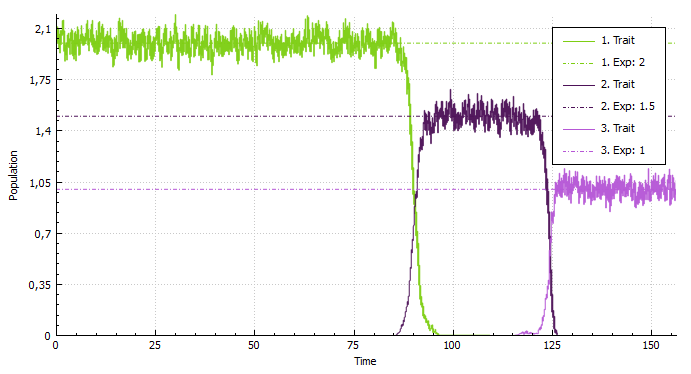
\includegraphics[width=0.8\linewidth]{./Pictures/TSS2_pure_small}
		\caption[TSS Approximation wechselnder Dominanz]{TSS-Approximation mit: K = 1000 und $ 4 \cdot 10^6 $ Sprüngen}
	\end{figure}
\end{frame}

\section{Simulation}
\begin{frame}{Simulation - Was und wie wird simuliert?}
	\begin{itemize}\pause
		\item Ein Sprung des BPDL-Prozesses (evolution step).\pause
		\item Implementation: Sorgf"altige Trennung der Aufgaben.\\
			Pseudocode: Gesamter Arbeitsablauf.\pause
%		\item "Ubersichtlich und mit transparentem Ablauf.\pause
	\end{itemize}
	Zun"achst wird die Implementation durch ein Diagramm verdeutlicht.
%	Folgend ist ein Diagramm zur kompakten Darstellung der Implementierung und anschlie"send der Pseudocode in zwei Teilen.
\end{frame}

\subsection{Implementierung}
\begin{frame}
	\begin{figure}[H]
		\centering
		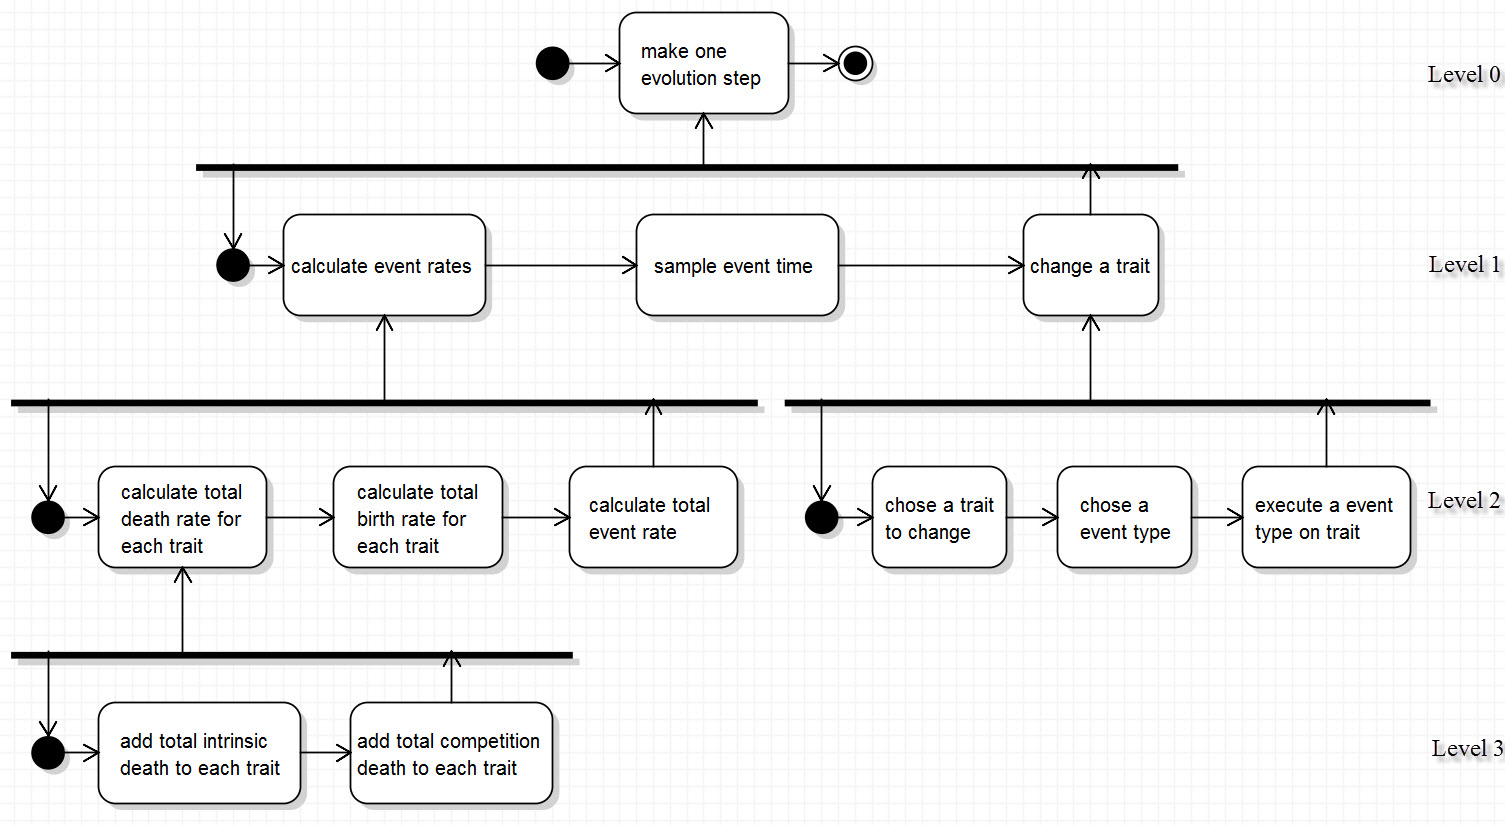
\includegraphics[width=1\linewidth]{../UMLs/PseudoCodeForBThesis}
		\caption{Diagramm mit Funktionsaufrufen und ihren Tiefenebenen}
	\end{figure}
\end{frame}

\subsection{Pseudocode}
\begin{frame}
	\begin{figure}[H]
		\centering
		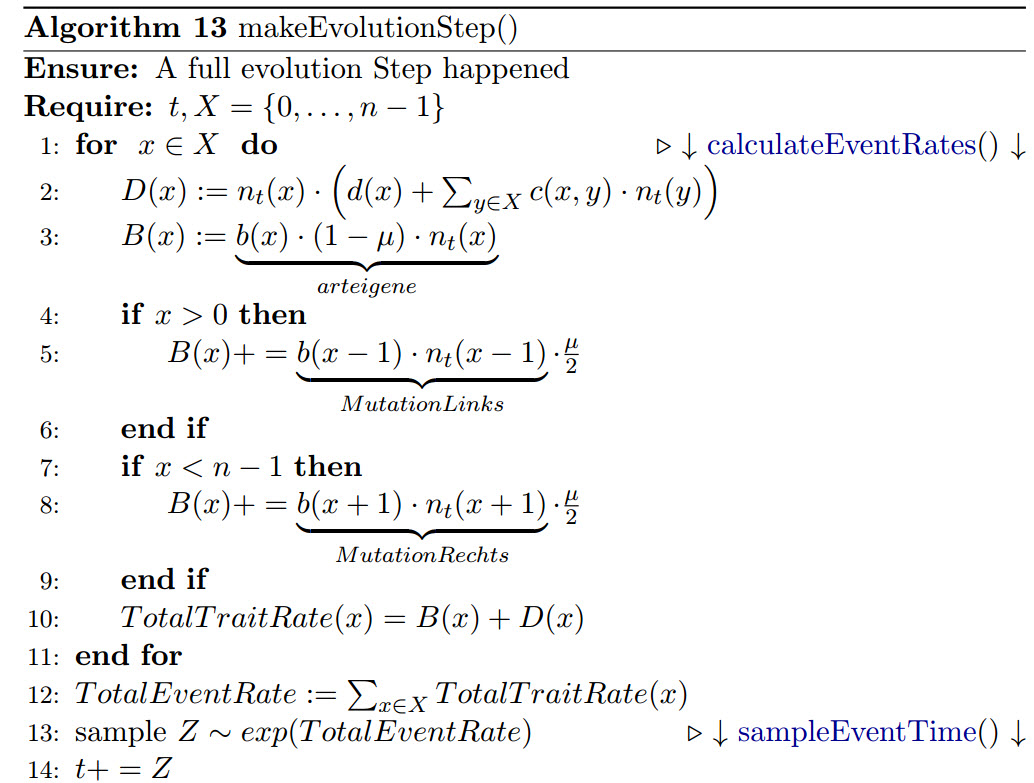
\includegraphics[width=1\linewidth]{./Pictures/Alg1}
	\end{figure}
\end{frame}
\begin{frame}
	\begin{figure}[H]
		\centering
		\includegraphics[width=1\linewidth]<1,3->{./Pictures/Alg2}
		\includegraphics[width=1\linewidth]<2>{./Pictures/SelectTrait}		
	\end{figure}
\end{frame}

\subsection{Optimierung}
\begin{frame}{Viele Merkmale?}
Bisher ist der Aufwand linear in der Anzahl der Spr"unge, doch quadratisch in Abh"angigkeit der Merkmale.\pause Daf"ur wurde in der BA eine Optimierung vorgestellt:
	\begin{itemize}
		\item Den gr"o"sten zeitlichen Aufwand fordert die Berechnung der Raten. Idee: Vermeidung der Neuberechnung.\pause
		\item Anpassung der Raten nach eintreten eines Ereignisses! Schritt beginn mit Ausf"uhrung der aktuellen Raten.\pause
	\end{itemize}
Dadurch l"asst sich linearer Aufwand erzielen.
\end{frame}

\begin{frame}{Viele Spr"unge und Normalisierung?}
Gerade mit gro"sem K werden viele Spr"unge notwendig. Diese werden schnell den Speicher "uberfluten.\pause\bigskip\\
Daf"ur wurden zwei L"osungen entwickelt und implementiert:\\
$ \rhd $ "{}erweiterte Spr"unge"{} - Speicherung von Messpunkten\\
$ \rhd $ "{}Storage"{} - Eine ausgelagerte tempor"are Datei\bigskip\\\pause
Wo wird eigentlich die Normalisierung angewendet?\\\pause
$ \rhd $ Kein Einfluss auf den evolution"aren Mechanismus.\\
$ \rhd $ Beim Einlesen und bei Zugriffen.\\
\end{frame}

\section{Programm}
\begin{frame}
	\frametitle{Arbeitsmodule}
	Die Architektur besteht aus 3 Modulen
	\pause
	\begin{figure}[H]
		\centering
		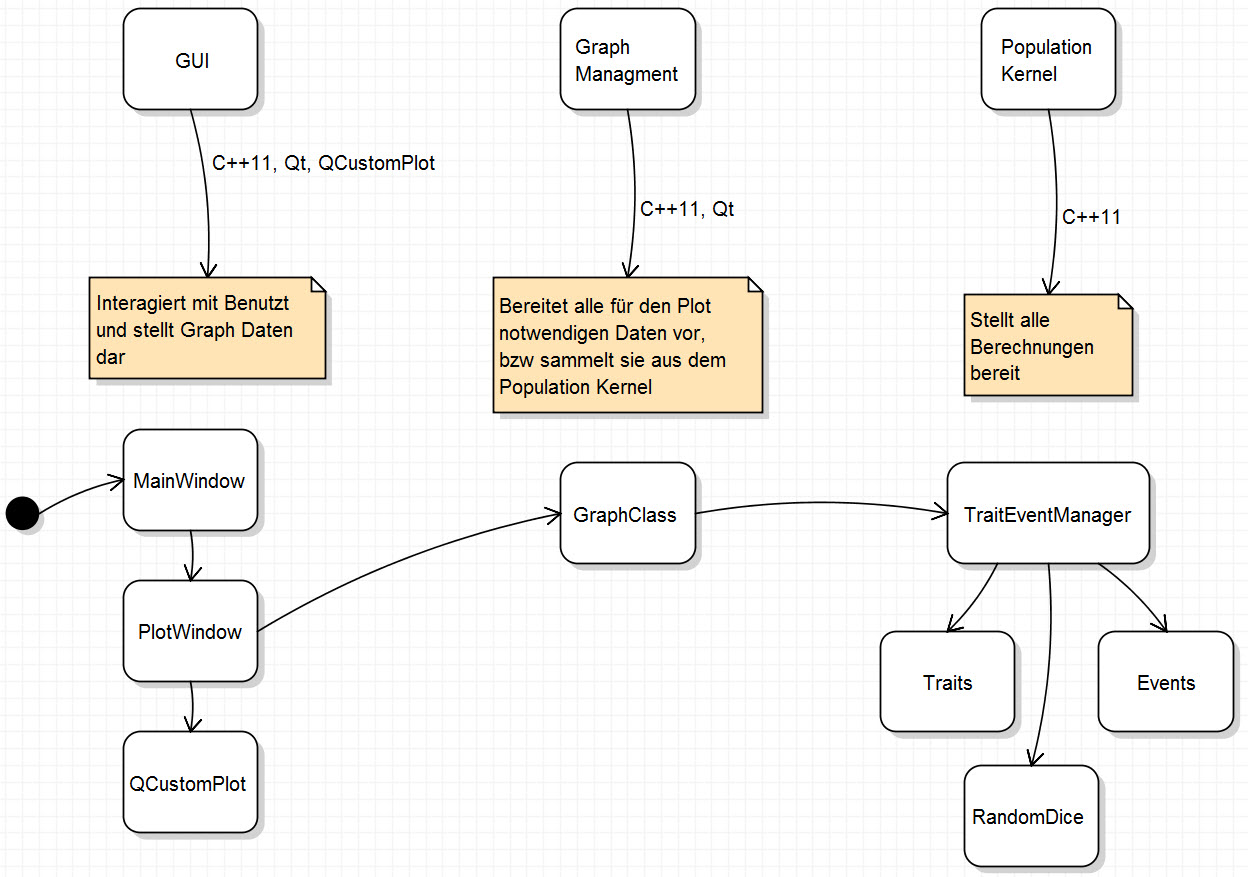
\includegraphics[width=0.8\linewidth]{./Pictures/Bild_Module}
		\caption[Module]{Arbeitsmodule und Klassenabhängigkeiten}
		\label{Module und Klassen}
	\end{figure}
\end{frame}

\subsection{Parameter}
\begin{frame}{Start}
	\begin{minipage}{1\textwidth}
		\begin{figure}[H]
			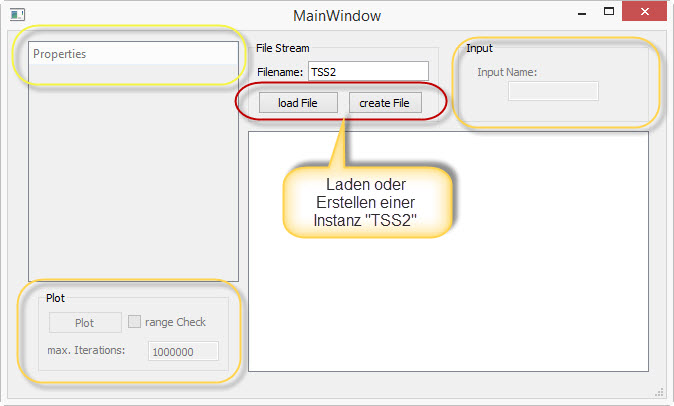
\includegraphics[width=1\linewidth]{./Pictures/MainWindow_Start}
			\caption[Startwindow]{MainWindow nach dem Start}
		\end{figure}
	\end{minipage}
\end{frame}
\begin{frame}{Lade Parameter}
	\begin{minipage}{0.45\textwidth}
		\begin{figure}[H]
			\centering
			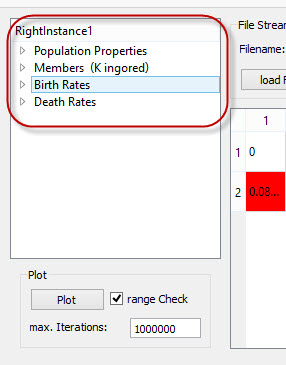
\includegraphics[width=1\linewidth]{./Pictures/MainWindow_ParameterBaum_zu}
			\caption[MainWindow_Parameter]{Baumstruktur - geschlossen}
			\label{Baumstruktur_geschlossen}
		\end{figure}
	\end{minipage} $ \quad $
	\begin{minipage}{0.45\textwidth}
		\begin{figure}[H]
			\centering
			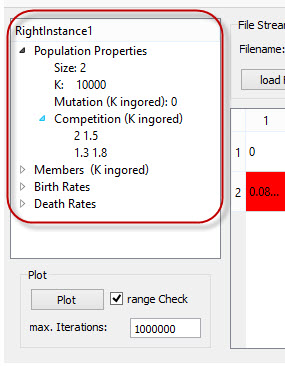
\includegraphics[width=1\linewidth]{./Pictures/MainWindow_ParameterBaum_offen}
			\caption[MainWindow_Parameter]{Verzweigte Baumstruktur - geöffnet}
			\label{Baumstruktur_offen}
		\end{figure}
	\end{minipage}
\end{frame}
\begin{frame}{Erstelle Parameter}
	\begin{figure}[H]
		\centering
		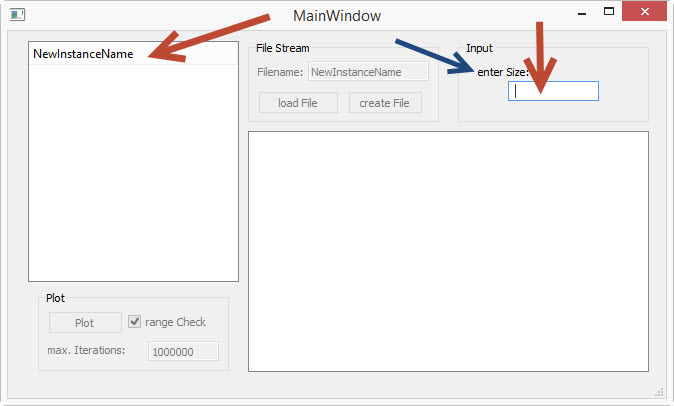
\includegraphics[width=1\linewidth]{./Pictures/MainWindow_createFile}\bigskip\\
		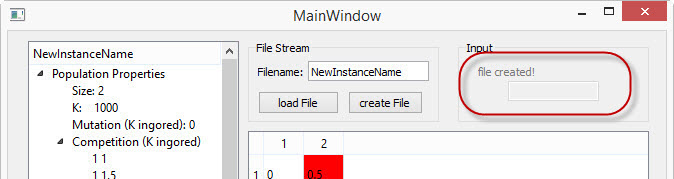
\includegraphics[width=1\linewidth]{./Pictures/MainWindow_FileCreated}
	\end{figure}
\end{frame}

\subsection{Darstellung}
\begin{frame}{Graphische Darstellung}
	An die graphische Darstellung wurden folgende Anforderungen gesetzt:
	\begin{itemize}
		\item Man soll den zeitlichen Verlauf der Populationsgrößen beobachten \- können.\pause
		\item Um die Prozesse besser analysieren zu können, soll es möglich sein, Stellen des Graphen näher betrachten zu können (zoom).\pause
		\item Um Simulationen vergleichen zu können, sollen außerdem Ausschnitte als Bilder gespeichert werden können.\pause
		\item Und natürlich soll das Programm bei der Berechnung nicht abstürzen.
	\end{itemize}
\end{frame}

\begin{frame}{Multithreading}
	Der letzte Punkt ist bei der Ereignisgesteuerten Programmierung tats"achlich eine nicht triviale H"urde. Daf"ur m"ussen Threads verwendet werden.
	\visible<2->{Dabei muss auf einige Punkte geachtet werden, z.B.:}\smallskip\\
	\begin{minipage}{0.49\textwidth}
	\begin{itemize}
		\visible<3->{\item Konfliktfreies Arbeiten (nicht Ereignisgesteuert).}
		\visible<4->{\item Race Conditions.}
		\visible<5->{\item Deadlocks (Endlos warteschleife).}
	\end{itemize}
	\end{minipage}
	\begin{minipage}{0.49\textwidth}
	\begin{figure}[H]
		\includegraphics[width=1\linewidth]<1->{./Pictures/KeineRueckmeldung}
	\end{figure}
	\end{minipage}\\\smallskip
	\visible<6->{Die L"osungen sind sogar bei erkanntem Problem nicht immer einfach zu finden. Bsp. Philosophenproblem.}
	
\end{frame}

\begin{frame}{Plot}
	In blau sieht man, dass das Programm durch Übereinanderlegen während der Berechnung weiterhin ansprechbar ist statt keine Rückmeldung zu liefern.
	\begin{figure}[H]
		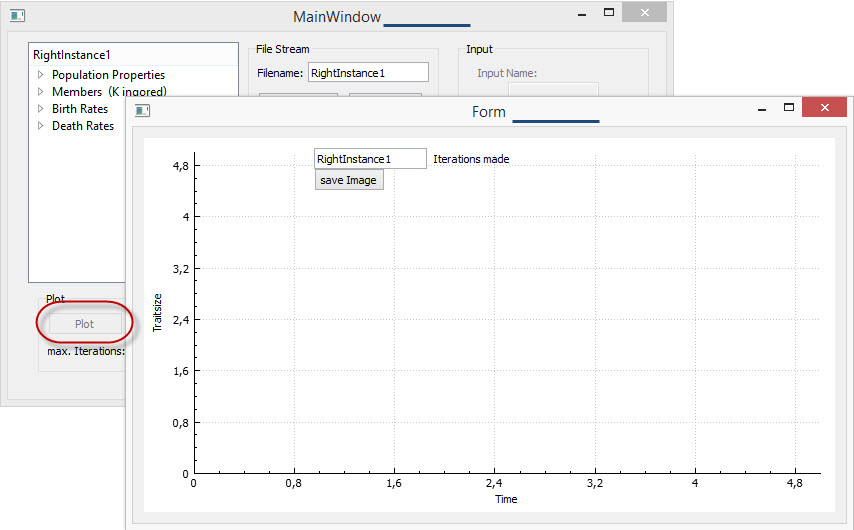
\includegraphics[width=0.75\linewidth]{./Pictures/PlotWindow_start}
		\caption[PlotWindow_start]{Start des PlotWindow}
	\end{figure}
\end{frame}

\begin{frame}{Plot}
	Nach der Berechnung, werden die Punkte verbunden. Das Ergebnis sieht folgenderma"sen aus:
	\begin{figure}[H]
		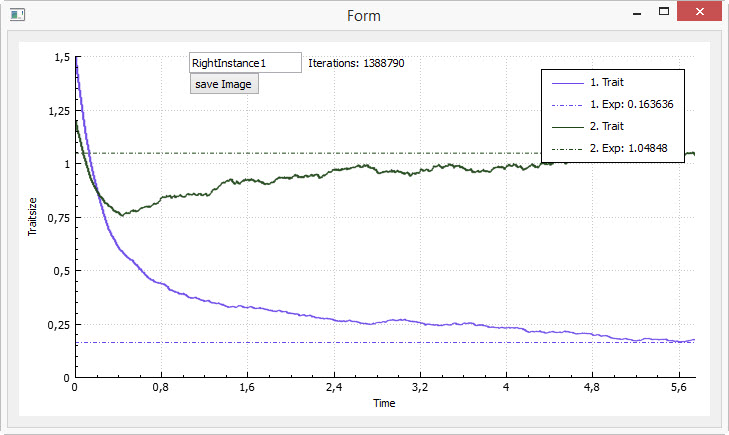
\includegraphics[width=0.85\linewidth]{./Pictures/PlotWindow_smallBPDL}
		\caption[PlotWindow]{PlotWindow mit Dimorpher Population}
	\end{figure}
\end{frame}

\begin{frame}{Optionen}
	Was bietet die graphische Darstellung?\smallskip\\\pause
	\begin{minipage}{0.42\textwidth}
	\begin{itemize}
		\item zeitliche Entwicklung.
		\item stabile Zust"ande.
		\item ben"otigte Spr"unge.
		\item Legende der Graphen.
		\item speichern des Bildes.
	\end{itemize}
	\end{minipage}
	\begin{minipage}{0.56\textwidth}
	\begin{figure}[H]
		\centering
		\includegraphics[width=0.9\linewidth]<4->{./Pictures/PlotWindow_zoomedBPDLmaximized}
	\end{figure}\pause
	\end{minipage}\smallskip\\
	Des weiteren lasst sich das Bild manipulieren:\pause
	\begin{itemize}
		\item Zoom mit automatisch anpassbarem Messgitter.
		\item Bewegung durch Ziehbewegungen.
		\item freie Skalierbarkeit des Bildes.
	\end{itemize}
\end{frame}

\section{Verhaltenstests}
\begin{frame}{Testgetriebene Entwicklung}
Die Korrektheit der Implementation ist zunehmend schwer zu pr"ufen (besonders bei pseudozuf"alligen Ereignissen).\\\pause
Was ist TDD und was tut ein Unit Test?
\begin{itemize}
	\item Eine Funktion die erwartetes Verhalten mit der Implementierung vergleicht.
	\item gew"ahrleisten Bedingungen um "Anderungen und Funktionalit"at so souver"an wie m"oglich zu gestalten.
\end{itemize}\pause
Aber warum sollten solche Tests Korrektheit des Programms gew"ahrleisten?
\end{frame}

\begin{frame}{Korrektheit}
$ \rhd $ Korrektheit und Flexibilität, f"ur alle Instanzen nachzuweisen ist schwierig.\smallskip\\\pause
$ \rhd $ Die jedes einzelnen Arbeitsschrittes jedoch weniger.\smallskip\\\pause
$ \rhd $ Arbeitsschritte sind sehr kurz und erf"ullen stets nur eine Aufgabe. Sie zu testen ist denkbar simpel.\smallskip\\\pause
$ \rhd $ Bei erfolgreichen Tests, wird bei richtiger Verwendung der Arbeitsschritte ein erwartetes Verhalten eintreten.\smallskip\\\pause
$ \rhd $ Die richtige Verwendung l"asst sich stets "ubersichtlich anhand des Algorithmus pr"ufen und wird nicht komplexer.\smallskip\\\pause
$ \rhd $ Daraufhin liefert die Unabh"angigkeit der Spr"unge die Gewissheit f"ur Folgespr"unge. \smallskip\\\pause
Damit ist die Komplexit"at der Simulation vereinfacht auf die der Ablaufpunkte.
\end{frame}

\section{TSS}
\begin{frame}{Invasion}
Schlie"slich kommen wir nochmal zu den TSS-Prozessen und unserer Approximation.\pause
	\begin{itemize}
		\item Wie bereits erw"ahnt bildet sich der TSS-Prozess im Grenzwert mit $ K\to \infty $ und $ \mu \to 0 $. Dadurch wird das sonst deterministische Verhalten stets durch zuf"allige Mutationen beeinflusst.\pause
		\item Die zuf"alligen Mutationen k"onnen eine Invasion ausl"osen. (Richtungsbedingt)\pause
		\item Der Bereich f"ur $ \mu $ garantiert Zeit zum Sterben und mutieren.\pause
		\item Invasionswahrscheinlichkeit resultiert aus der Fitnessfunktion: $ \frac{\left[ f(y,x)\right]_+ }{b(y)} $ (Anteil der Ereignisse)
	\end{itemize}
\end{frame}

\begin{frame}{Phasen einer Invasion}
	Sei $ f(y,x) > 0 $ und $ f(x,y) < 0 $.\smallskip\\
	\begin{minipage}{0.49\textwidth}
		\begin{itemize}
			\visible<1->{
			\item Fixierung: Kaum Auswirkung bis zu einer Populationsgr"o"se $ \varepsilon $
			\item Invasion: Verdr"angungsphase
			\item Aussterben: Unterschreitung der Populationsgr"o"se}
		\end{itemize}
	\end{minipage}
	\begin{minipage}{0.49 \textwidth}
	\begin{figure}[H]
		\includegraphics[width=1 \linewidth]<1>{./Pictures/Invasion2}
		\includegraphics[width=1\linewidth]<2->{./Pictures/MainWindow_red_green_loaded}
	\end{figure}
	\end{minipage}
\end{frame}

\begin{frame}{Optimierung}
	Normalerweise verbringt die Simulation der TSS-Approx\-imation viel Zeit im monomorphen Gleichgewicht.\\
	Dabei l"asst sich nicht gut nachvollziehen ob sich etwas ereignet.\bigskip\pause\\
\begin{minipage}{0.59\textwidth}
	\includegraphics[width=1\textwidth]<2>{./Pictures/TSS2_pure_small}
	\includegraphics[width=1\textwidth]<3,4>{./Pictures/TSS2_optimierung_small}
	\includegraphics[width=0.35\textwidth]<5>{./Pictures/TSS_DomZoomVgl_original}
	\includegraphics[width=0.35\textwidth]<5>{./Pictures/TSS_MutationZoomVgl2_original}	
	\includegraphics[width=1\linewidth]<6->{./Pictures/TSS_MutationZoom2_original}
\end{minipage}	
\begin{minipage}{0.39\textwidth}
\begin{itemize}
	\visible<3->{\item Lineare Interpolationen in g"unstigen Bereichen.}
	\visible<4->{\item Verbessert "Ubersichtlichkeit, Analyse und Laufzeit.}
	
\end{itemize}
\end{minipage}\\
\end{frame}

\begin{frame}{Implementierung}
	\begin{algorithm}[H]
		\caption{isNear()}
		\begin{algorithmic}[1]
			\Ensure{Bedingungen für eine Interpolation}
			\For{ i = 0 $ < $ n-1}
				\If{i $ \ne $ ChosenTrait \& Members[i] $ > 0 $}
					\State \Return false;
				\EndIf
			\EndFor
			\If{$ |\text{getKMembersOf[i]} - \text{Expected[ChosenTrait]}| > \frac{0.5}{K} $}
				\State \Return false;
			\EndIf
			\State \Return true;
		\end{algorithmic}
	\end{algorithm}
\end{frame}

\begin{frame}{Ende}
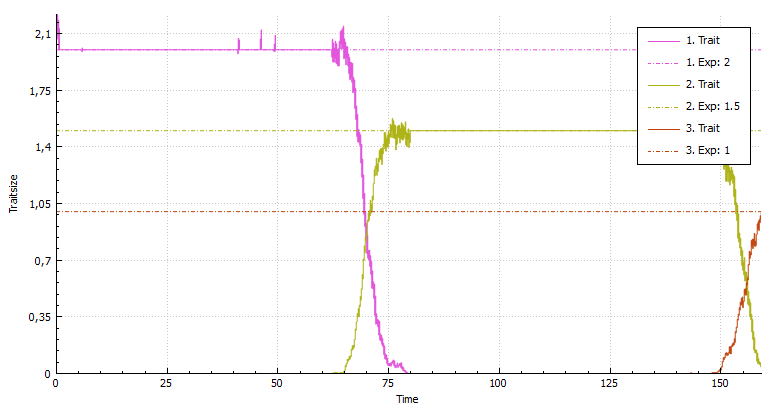
\includegraphics[width=1\textwidth]{./Pictures/TSS2_optimierung_small_original}
\end{frame}
\end{document}
% ä Ä ö Ö ü Ü